% !TEX TS-program = pdflatex
% !TEX encoding = UTF-8 Unicode

% This is a simple template for a LaTeX document using the "article" class.
% See "book", "report", "letter" for other types of document.

\documentclass[11pt]{article} % use larger type; default would be 10pt

\usepackage[utf8]{inputenc} % set input encoding (not needed with XeLaTeX)

%%% Examples of Article customizations
% These packages are optional, depending whether you want the features they provide.
% See the LaTeX Companion or other references for full information.

%%% PAGE DIMENSIONS
\usepackage{geometry} % to change the page dimensions
\geometry{a4paper} % or letterpaper (US) or a5paper or....
\geometry{margin=1in} % for example, change the margins to 2 inches all round
% \geometry{landscape} % set up the page for landscape
%   read geometry.pdf for detailed page layout information

\usepackage{graphicx} % support the \includegraphics command and options

% \usepackage[parfill]{parskip} % Activate to begin paragraphs with an empty line rather than an indent
\usepackage{amssymb}
\usepackage{amsmath}
%%% PACKAGES
\usepackage{booktabs} % for much better looking tables
\usepackage{array} % for better arrays (eg matrices) in maths
\usepackage{paralist} % very flexible & customisable lists (eg. enumerate/itemize, etc.)
\usepackage{verbatim} % adds environment for commenting out blocks of text & for better verbatim
\usepackage{subfig} % make it possible to include more than one captioned figure/table in a single float
% These packages are all incorporated in the memoir class to one degree or another...

%%% HEADERS & FOOTERS
\usepackage{fancyhdr} % This should be set AFTER setting up the page geometry
\pagestyle{fancy} % options: empty , plain , fancy
\renewcommand{\headrulewidth}{0pt} % customise the layout...
\lhead{}\chead{}\rhead{}
\lfoot{}\cfoot{\thepage}\rfoot{}

%%% SECTION TITLE APPEARANCE
\usepackage{sectsty}
\allsectionsfont{\sffamily\mdseries\upshape} % (See the fntguide.pdf for font help)
% (This matches ConTeXt defaults)

%%% ToC (table of contents) APPEARANCE
\usepackage[nottoc,notlof,notlot]{tocbibind} % Put the bibliography in the ToC
\usepackage[titles,subfigure]{tocloft} % Alter the style of the Table of Contents
\usepackage{bbm}
\usepackage{endnotes}

\renewcommand{\cftsecfont}{\rmfamily\mdseries\upshape}
\renewcommand{\cftsecpagefont}{\rmfamily\mdseries\upshape} % No bold!
\DeclareMathOperator*{\argmax}{arg\,max}
\DeclareMathOperator*{\argmin}{arg\,min}

\usepackage{graphicx}
\graphicspath{ {./pings/} }

\newcount\colveccount
\newcommand*\colvec[1]{
        \global\colveccount#1
        \begin{pmatrix}
        \colvecnext
}
\def\colvecnext#1{
        #1
        \global\advance\colveccount-1
        \ifnum\colveccount>0
                \\
                \expandafter\colvecnext
        \else
                \end{pmatrix}
        \fi
}

\newcommand{\norm}[1]{\left\lVert#1\right\rVert}

\title{IO Problem Set 4}
\author{Michael B. Nattinger}

\begin{document}
\maketitle

At the end of the document I present a series of screenshots of the Stata output. I was going to present nicely formatted tables instead but I don't have the time. Still, all of the information one would expect in the tables should be represented by the output.


\section{Question 1: Probit entry}

For the Walmart entry probit, I found the following specification to perform the best: Kmart presence, log of county population, log of retail sales, percent of urban population, log distance to Benton, Southern (dummy), number of small stores, and distance weighted num of Kmart stores.

For the Kmart entry probit, the optimal model was similar: Walmart presence, log of county population, log of retail sales, percent of urban population, Midwest (dummy), log distance to Benton, and Southern (dummy).

The model is blind to entry of Walmart into a country that already has a Walmart. This is probably a bad assumption, as Walmart presence will have a massive impact on Walmart entry into a country, as Walmart will try to reduce competition for themselves.

Also, we are proxying for entry with presence in a market. These concepts of course are related, but not the same.

\section{Question 2: Probit}
As requested, we use the variables we excluded in Question 1 as instruments here. Technically speaking, we should not use distance from Benton county as an instrument as it was not excluded in Question 1. Benton is where Walmart is headquartered so it may directly influence Walmart's decision but not Kmart's, so it may only affect Kmart through its influence on Walmart. That being said, I think the 'Southern' dummy is going to suck up a lot of the variation from this variable as Benton county is in Arkansas. We could potentially take it out of Kmart's regression from Question 1 and use it as an instrument in Kmart's part of problem 2, I suppose.

\section{Question 3}
Here we do the Bresnahan and Reiss stuff. One problem here is that we are thinking of Big vs Small players but the only big players we are considering are Walmart and Kmart? This is a bad assumption and influences our results dramatically. This is a big-time limitation.

\section{Question 4}

Here I applied the two-step: Probit with entry of Walmart as dependent variable, then estimate Walmart entry probabilities. These probability estimates are then used in the second stage regression where Kmart entry is the dependent variable and Walmart probabilities are included as a covariate. We also do the opposite, where we look at Probit regression with Kmart entry as dependent variable in first-stage, then in second stage incuded probability estimates from first stage as explanatory variables in the second stage regression, where Walmart entry is the dependent variable.

These results indicate that the entry of the other player in the market has a massive influence on the entry decisions of a player. Much more than other sections. When the other firm enters, it reduces my profits from entering, and such reduces my probability of entry.

\section{Stata Output}
Here is all of the content of the pset. I will include all of my code in with my Canvas submission. Sorry if it is not that well organized, my TA position is absolutely ruining my life right now.

\begin{center}
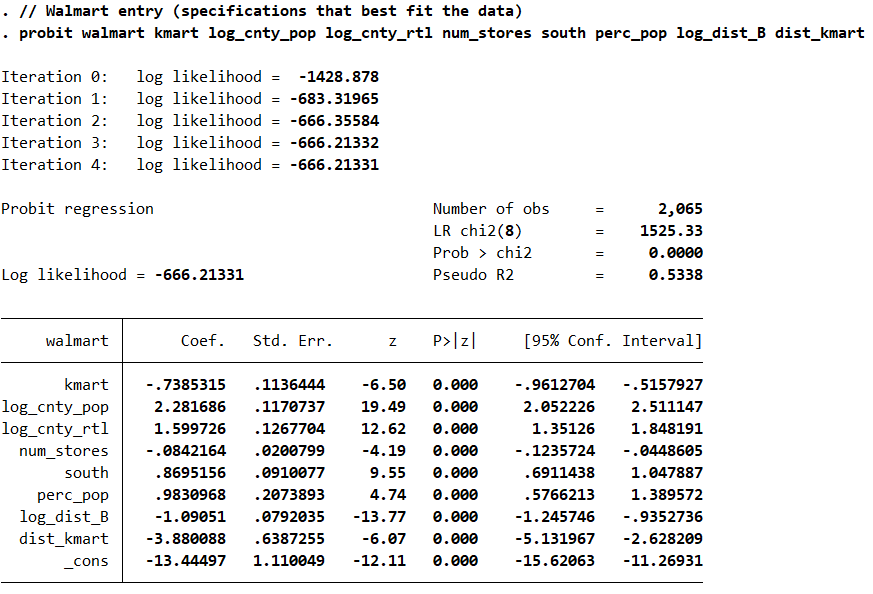
\includegraphics{fig1}

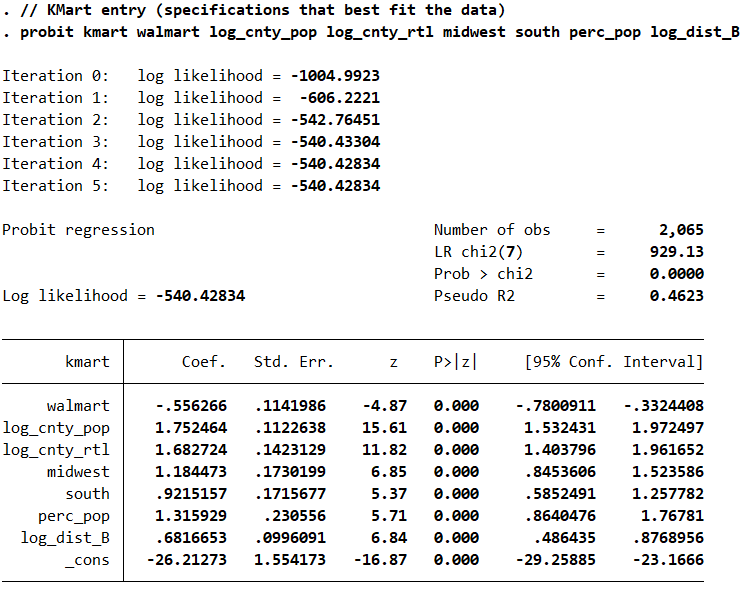
\includegraphics{fig2}

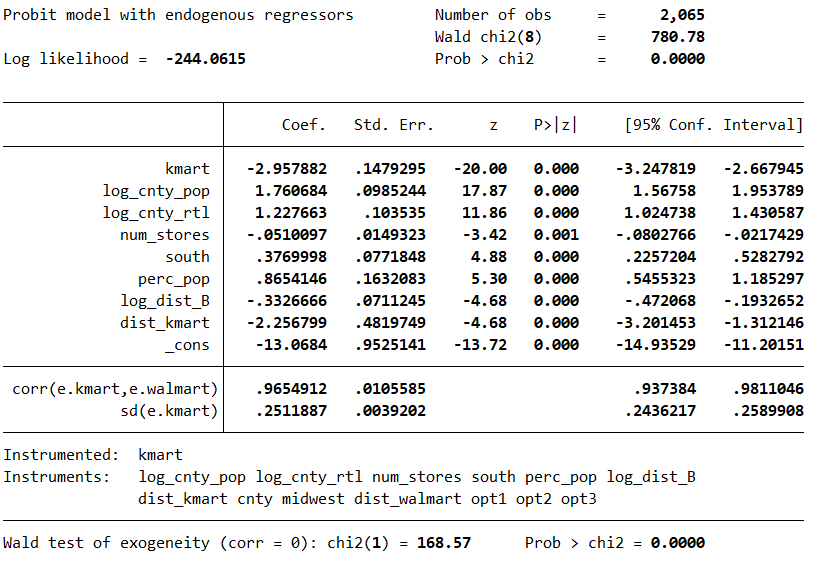
\includegraphics{fig3}

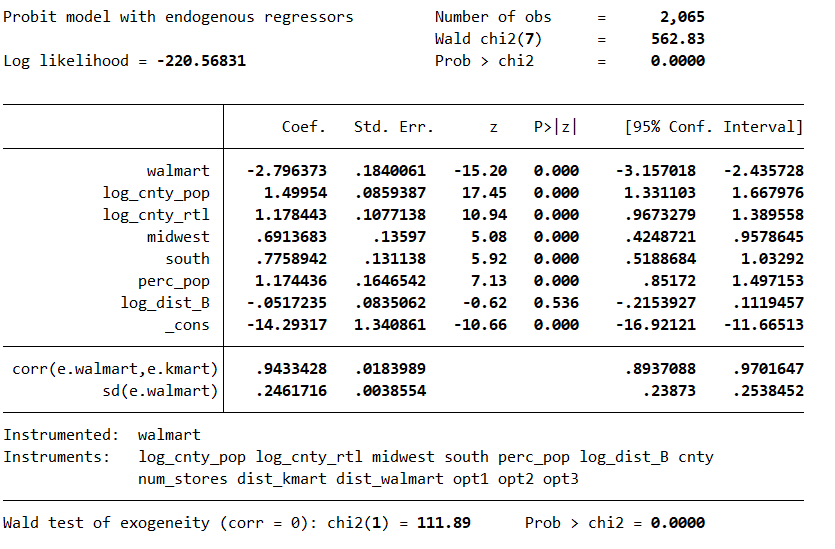
\includegraphics{fig4}

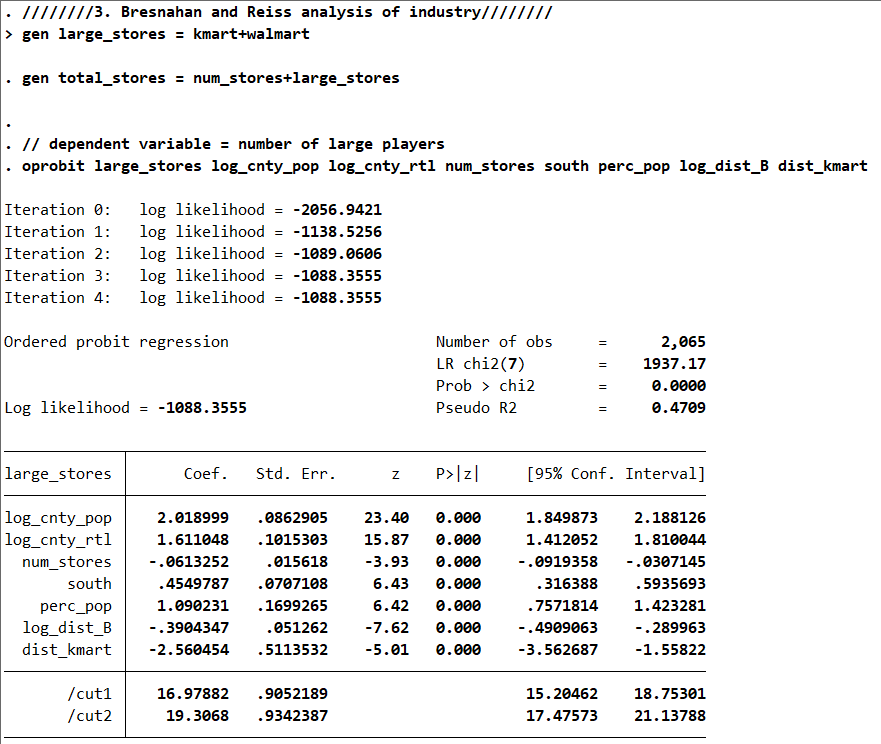
\includegraphics{fig5}

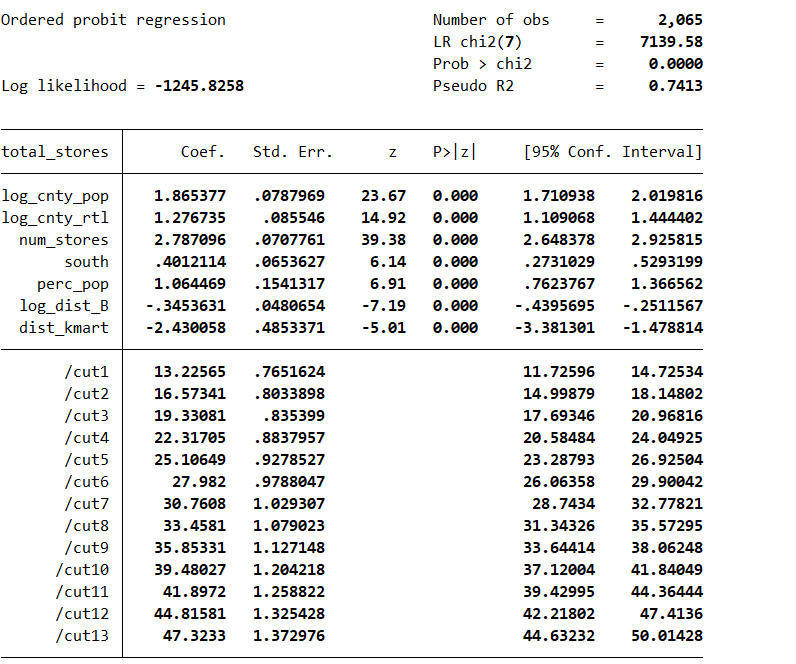
\includegraphics{fig6}

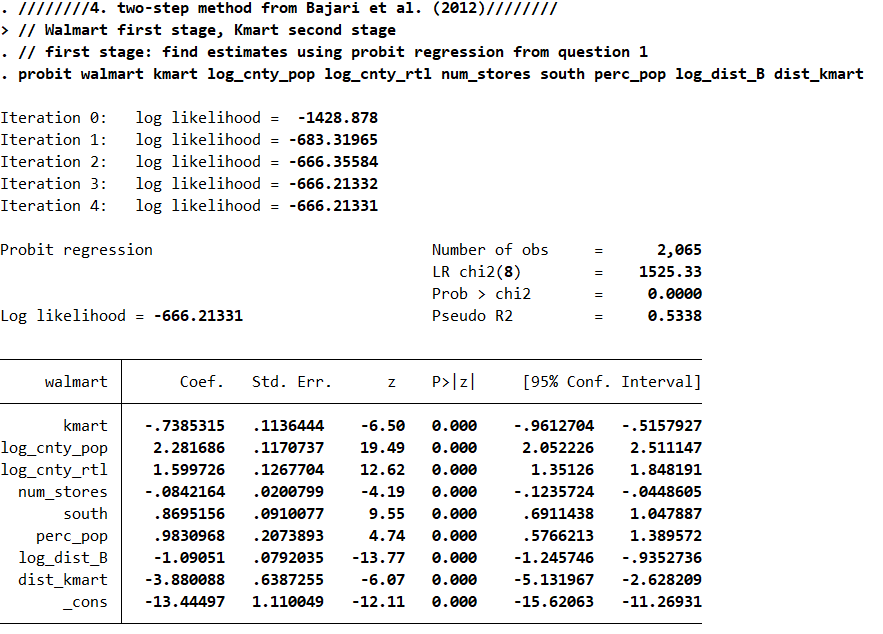
\includegraphics{fig7}

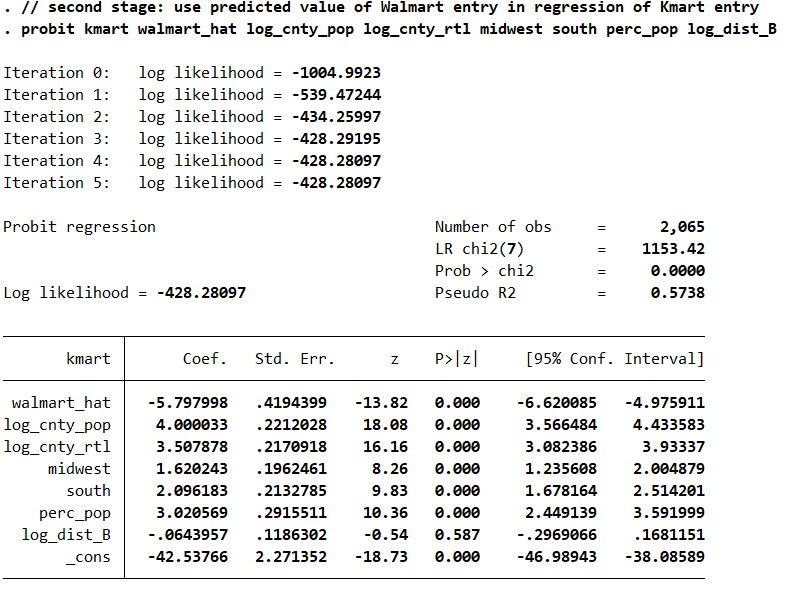
\includegraphics{fig8}

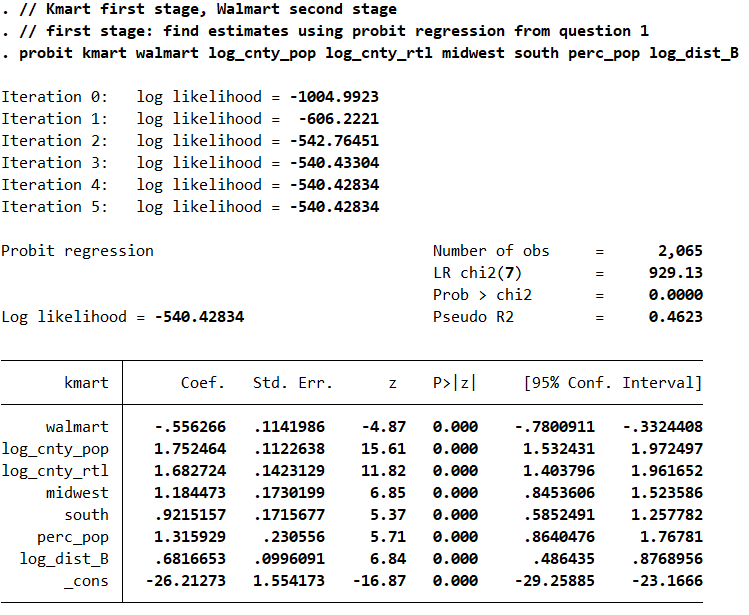
\includegraphics{fig9}

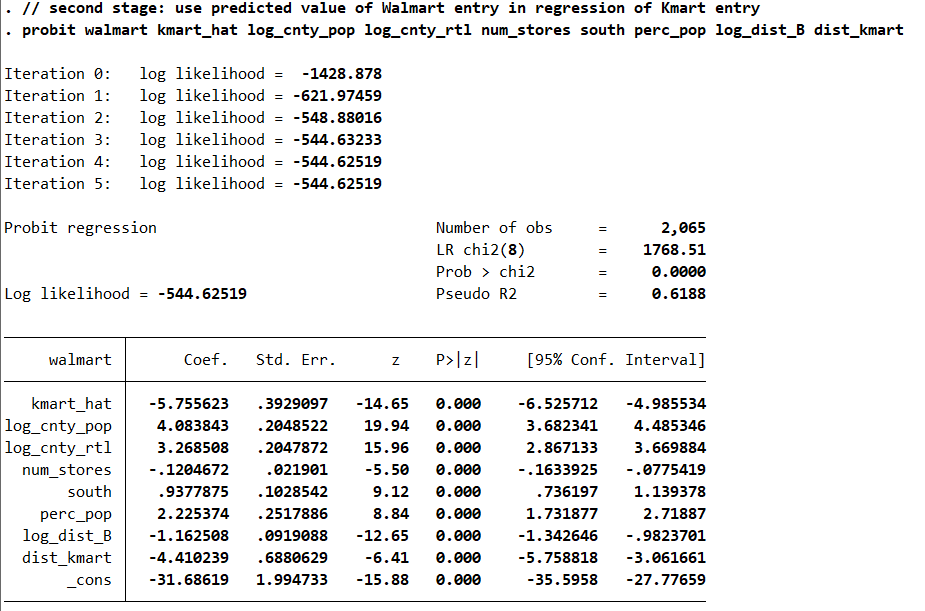
\includegraphics{fig10}

\end{center}
\end{document}
